%\documentclass{tufte-handout}
\documentclass{article}
\usepackage{amsmath,amsthm}
\usepackage{fontspec}
\usepackage{float}
%\usepackage{unicode-math}
%\setmathfont{Palatino Linotype}
%\setmainfont{Palatino Linotype}
%\usepackage{minted}
%\usemintedstyle{bw}
\usepackage{hyperref}

%\input{vc.tex}

%\newtheorem{claim}{Claim}[section]
\title{Control of Batch Tank using Raspberry Pi \\ FRTN01 project - Group 20}
%\date{\GITDate,\\\small\GITAbrHash}
%\date{}
\author{Johan Anderholm \\ Jonathan Kämpe \\ Mikael Sahlström \\ Mikael Nilsson}

\begin{document}
\maketitle
\newpage
\tableofcontents
\newpage
\section{Problem description}
% An introduction that states the problem that has been solved.
This project aims to control a process called batchprocess that consists
of a water tank, two pumps (one for pumping into the tank and one for
pumping out of the tank), a heater, a cooler and a mixer. As stated in
the project descriptions \cite[p.~6]{project12}, we should
simultaneously control the level and temperature of the tank while at
the same time simulating an exothermic chemical reaction.

The heater will simulate an exothermic reaction and whenever the
temperature rises to high the in pump is used the in pump to lower the
water temperare. The out pump is used to keep the water level at a
reference level that can be set dynamically in a settings file for the
PID client that controls this pump.

The available sensors of the batchprocess is a water level meter and a
temperature meter.

The control system should be designed as a distributed system, i.e. it
should be possible to have geographically separate controllers connected
to the process via relatively low latency and stable networking. Parts
of the system should run on a small credit-card-sized computer called
Raspberry Pi.

\subsection{Raspberry Pi}
The idea is to be able to keep a server on a Raspberry Pi attached the
batch process. Thus creating a "movable" system. Also interacting with
the process is made platform and hardware independent. Designing
controllers should be possible over any hardware and any physical link
layer capable of TCP/IP.

The Raspberry Pi is a single chip computer running an Broadcom BCM2835
system on a chip including among other things an ARM11 CPU and a
floating point unit fully compliant with the IEEE 754 standard.


\section{Program structure}
% A section describing the main program structure, both from a class
% and and a real-time perspective. If possible illustrate this with some
% type of figure.
This project is designed as a two-tier client/server system 
\cite[p.~6]{clientserver} where none of the control processes need to be directly
connected to the batch tank.

The server consists of a driver that communicates with the batch tank over a
serial interface, and a part responsible for managing connections from
clients and serves them with desired data. The control signals from client are redirected to the driver which sends them to the batch tank. The communication
between the server and its clients is done via the TCP/IP protocol which means
that the clients can be located anywhere. In our tests we have had clients
running on the same device as the server and on separate devices connected
through a switch and TP-cable.

From a high level perspective the system is very similar to message
passing \cite[p.~71]{rtcs}. The server listens for messages, each
containing any number of the predefined events, and processes these as
soon as possible.

\begin{figure}[H]
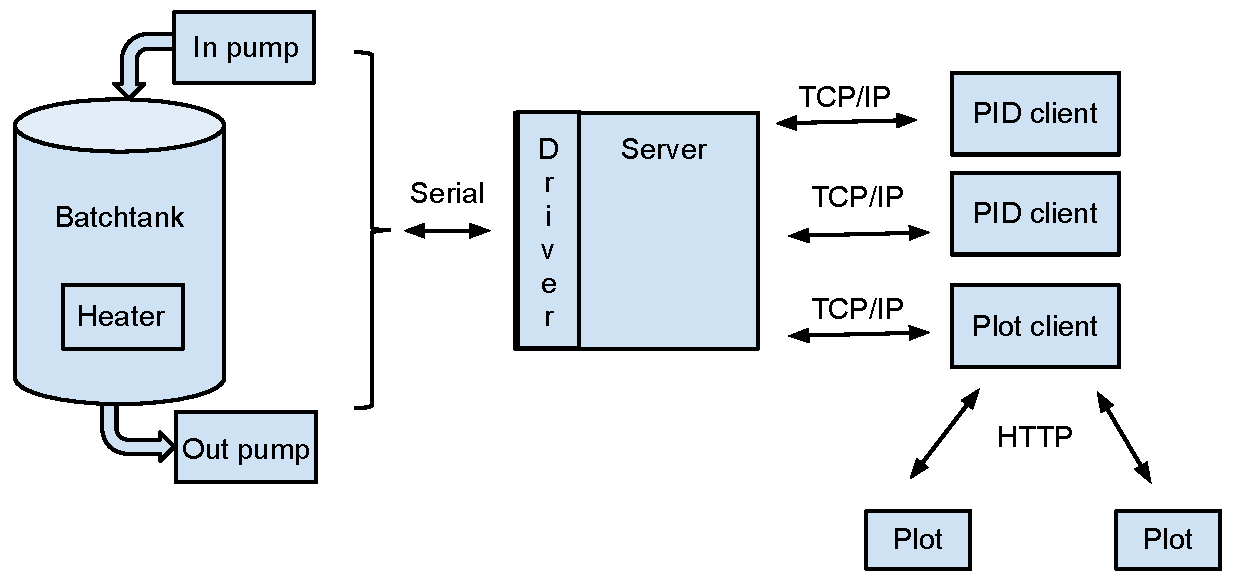
\includegraphics[width=0.9\textwidth]{systemoverview.pdf}
\caption{An overview of the program structure.}
\label{fig:system overview}
\end{figure}

\subsection{Events}
The following events are defined:

\begin{description}
\item[sample]
  A client may listen for sample events and from this produce a control
  signal. The sample message contain sensor type and the value of said
  sample.
\item[signal]
  The server listens for (control) signal events and uses these to
  control the batchtank process. A control signal message contains
  information on output to be used and the value as well as the
  reference value used to produce said signal.
\item[register]
  Upon receiving a register event, the server periodically samples the
  process and sends these samples to the client. Inside a register
  message period time and any number of sensors are defined.
\item[getSensor]
  Used to tell the server to respond with samples for any number of
  sensors right now, without any regard for the period time and such.
\item[getOutput]
  Similar to getSensor but responds with the latest used control signal
  (value and reference value) for specified output.
\end{description}

\subsection{External libraries}
\begin{itemize}
\item{jQuery}
\item{Flot}
\item{Boost}
\end{itemize}


\subsubsection{Protocol Buffers}
The messages used to communicate between clients and the servers are
described using a interface description language called Protocol
buffers, or protobuf \cite{protobuf}.

Messages are compiled into the language of choice resulting in a series
of classes and packages used to create the messages which then can be
serialized and sent over wire in binary format. It is designed for high
performance and small serialized size. The official protocol buffers
compiler is able to produce C++, Java and Python code. This project uses
C++ and Python successfully.

There are a few benefits to using Protocol Buffers over a hand written
binary protocol, or a language native serializing protocol. Language
native serialization requires using a specific language and is seldom as
efficient in terms of message size and serializing speed. A custom
binary protocol may require very large reworking of actual code in the
case of late stage changes.


\subsubsection{boost::thread~\cite{boost::thread}}
Originally the idea was to use the new C++11 threads. However there's
not yet very good support for that among compilers. Boost provides a
threading library very similar to that of std::thread and was used
instead. On posix platforms this equates to using POSIX threads in the
end.


\subsubsection{boost::asio~\cite{boost::asio}}
In order to simplify server and client communication in C++ a networking
library called Asio is used. While asios main goal is to provide a
consistent asynchronous network model it does contain good support for
synchronous networking as well. It is much easier to work with than
regular Unix socket, although at some level raw Unix sockets are being
used anyway.


\subsection{Server}
The server is implemented using C++ in order to run well on the Raspberry Pi as
there is currently not any acceptable JVM with proper JIT available. It
also makes calling timing functions more appropriate for real time tanks
considerably easier. The server consists of the following classes:

\begin{description}
\item[IORegistry]
  This class is used as an interface against the batchtank server.
  Mutexes are used in order to make reading and writing to the process
  atomic operations.

\item[ConnectionThread]
  Whenever a connection is made to the server a \verb+ConnectionThread+
  is fired and given control over that particular connection. Each
  connection contains a main reading loop executing controller events.
  It is running as a detached thread.

\item[PeriodicTask]
  Executes a function on a strictly regular basis. Uses
  \verb+clock_nanosleep+  with \verb+TIMER_ABSTIME+ and
  \verb+CLOCK_MONOTONIC+ and should have a fairly high resolution.

\item[Sampler]
  Ran as periodic task to sample at specified intervals.
\end{description}


\subsubsection{Use scenario}
The server listens to a port specified in a \verb+.ini+ file. When a client
connects the connection is assigned a dedicated \verb+ConnectionThread+. 
Upon a register event recieved a \verb+PeriodicTask+ is fired together
with a sampler that samples and sends samples to the client at a regular
interval. The register message contains data such as period time and
what sensors to read.

The client may respond with control signal events which specify what
value should be set as well as to what output. It also contains the
reference value used for this control signal.

Setting and getting values from the batch process is protected by a
\verb+IORegistry+ however locking of the registry is external, i.e. it
contains a public mutex and does no locking on its own. This is done in
order to enable batching several gets and sets as single atomic
operations. The \verb+IORegistry+ also contains copies of reference
values as well as control signals for plotting use cases.


\subsection{Driver}
The driver for the communication with the batch tank over a serial port is written in the C language.
It makes use of the Unix API for terminal I/O. The operative system's driver will
map the serial device to a file descriptor, hence the reads and writes are done
with standard C functions read(3), write(1), open(2) and close(2).  The serial
connection has a speed of 115200 baud. 

The driver has a set and get function and a couple of enumerators specifying the
sensor or motor to set or to get. The driver supports all available sensors or motors of
the batch tank; temperature, water level, in/out pump, mixer, cooler and heater.

The get function is blocking with a time out of 1 second. Any kind of failure will
make the functions return a negative number. Data is sent and received in chunks
of 8 bits. The get function sends a byte asking the batch tank to send some
information about a specific sensor or motor, it then blocks on the read function
until all bytes are read. The set function simply puts commands on the serial
line. The bytes are processed in accordance to the protocol description found in the source code that runs on the
batch tank \cite[line 150-223]{kokare.c}. 

The driver will always parse the whole value into bytes and then send it to the
batch tank. The batch tank only supports values between 0 and 255. The
temperature and the water level sensors may generate greater values than 255.
This is all supported. The driver is not thread safe.


\subsection{PID client}
The PID client, written in C++, consists of a main method which uses boost
libraries for communication with the server and a PID class with the following
public members:
\begin{itemize}
\item{void updateParameters(const PIDParameters\&);}
\item{double next(double);}
\item{void updateStates();}
\end{itemize}

The PID parameters include K, Ti, Td, Tr, N, ref, umin, umax, inverted, and 
period. Also, the client also takes parameters on server ip/port, which sensor
to read, and which item to control which makes the whole system easy to
configure and dynamic in adding/removing controllers.

It is possible to update the PID parameters on the fly by editing the 
\verb+.ini+ file.
The client will parse the parameters again whenever the unix signal USR1 is
received. An external python process is used to monitor the configuration file
and client process. It sends the signal when the file has been changed. The
monitoring is done using inotify.
Note that no error checking is done. I.e. the client crashes when asked
to update using a malformed configuration file. 

\subsubsection{Use scenario}
The client starts with parsing server and controller details from a
\verb+.ini+ file. After a successful connection the client registers for
samples by issuing a register event to the server. Sensor and period
is defined in register event and after this the client starts to wait
for sample events. When one is received a control signal is calculated
and sent as a signal event. Then controller states are updated and the
client starts to wait for the next sample event. The user can change the
PID parameters at any time in the \verb+.ini+ file. The program will 
reparse the file automatically.
 


\subsection{Plot client}
The plot client, written in Python \cite{python}, is in itself a server/client
system where the server is a client to the main server and the clients are web
browsers running the Javascript plotting code. When started, a HTTP server will
start serving a HTML and Javascript page which is to be run in a browser. This
page will request new data to plot from the HTTP server which then requests data
from the main server. The main server then sends data (such as water level,
control signals and reference signals) to the HTTP server which parses it into
JSON \cite{json} formatted data and sends it to the plot page. The data format is
as follows:
\begin{verbatim}
{"Plot name": { "Curve name": [y value, ...], ... }, ... }
\end{verbatim}
The data will be received and parsed by Javascript code which will go through it
step by step. First, the code checks if a plot exists and creates the plot if
not. Then if the curves exists in the plot and creates them if not. Then each y
value will be shifted onto the curve data, from the right. This data will
initially contain 100 zeros. The same amount of data that is shifted from the
right is shifted out from the left so that the curve always contains 100
data points. This will create an effect where the data flows from the right to
the left smoothly.


\subsection{Manual client}
There exist a Python client capable of manipulating the different parts
of the batch process. It is realized as a class containing properties
such as \verb+mixer+, \verb+heter+, \verb+level+. By importing this into
a interactive shell such as \emph{IPython} manual control is effectively
accomplished.


\section{Control design}
% A section describing the control design aspects of the project.
The controller is a standard PID controller implemented with forward
approximation integral, backward approximation derivative, bumpless transfer,
and tracking as anti-windup. The temperature of the system is controlled with
the in pump and the water level is controlled with the out pump.
The parameters have been chosen by empirical
studies and are displayed in table \ref{paramtable}. The reference value of the
in pump PID should be adapted to the temperature of the water reservoir so the 
cooling procedure is not too easy or hard. A wanted temperature which is less
than the temperature of the water will obviously never be reached without using
the cooling element. The chemical reaction is simulated by a PID. Note that the
settings of this PID will read create a control signal which
is $K*temp$ and feed it to the heater. This will create an accelerating 
temperature when K is large enough. 

The control loop does the following in one iteration.
\begin{itemize}
\item{Wait for y}
\item{Calculate u}
\item{Send u}
\item{Update states}
\end{itemize}

\begin{table}[h]
\begin{tabular}{|l|l|l|l|l|l|l|l|l|l|l|l|}
\hline
PID      & Sensor & period (ms) & K & Ti & Td & Tr & N & ref & umin & umax & inv \\
\hline
In pump  & TEMP & 50 & 10 & 10 & 0 & 1 & 0 & 370 & 0 & 200 & true \\
\hline
Out pump & LEVEL & 50 & 3 & 2 & 0 & 2 & 0 & 400 & 0 & 255 & true \\
\hline
Reaction & TEMP & 50 & 0.6 & 0 & 0 & 0 & 0 & 0 & 0 & 255 & true \\
\hline
\end{tabular}
\caption{\small{This table shows the parameters used for the PID clients.
		 when inv is set the error will be negated.}}
\label{paramtable}
\end{table}

\section{Running the system}
% A section describing the user interface in the project including a short
% HowTo description on how to start and operate the program.
The source code of the system is publically available in a GitHub
repository~\cite{repo} and can be retrieved using GIT or as a zip archive.
The different part of the system is divided into the following directories:
\begin{description}
\item[server]
  TCP server used for manipulating the actual process.
\item[pid\_client]
  TCP client PID regulator.
\item[manual\_client]
  Python client/library used for connecting to the server and manipulating the
  batch process directly.
\item[plot\_client]
  Python based http\_server and client used for serving plotting data.
\item[cook]
  C library for serial communication to the actual batch process.
\item[proto]
  Protocol buffer definition.
\item[common]
  C++ utility functions shared between client and server.
\end{description}

Each part is described more in depth in its corresponding directory.

To start the system one should first connect a device to the batch tank.
During development a serial to USB adapter was used but as long as the
correct port is specified in \emph{batchtank\_server.ini} anything
should work.

After connecting the device to the batch tank start batchtank\_server and it will
start listening for incoming TCP connections from clients. Run these on either
the same device as the server or on separate devices connected, via TCP/IP, to
the server. Note that depending of the permissions of the serial port
the server may require super user privileges.

\section{Results}\label{results}
% A section containing the results. In case the project is a control-oriented
% project this should include plots of measurement signals, reference sig-
% nal, and control signal. If the project is more of a real-time nature then
% this section could contain measurement results of different type.
In all our tests we can see that the water level have a "high frequency" noise
that comes from when the water stream from the in pump hits the water in the
tank. This noise is reflected upon the control signals that are based on water
level measurements and can be seen in figure~\ref{fig:out pump}. 

The high frequency noise does not affect the pumping power so much as they can not make such small and frequent changes in power.

When the derivative part of the controller was used a more unstable system  was
observed.

Figure~\ref{fig:out pump} shows how a PID client controlling the out pump reacts
to a change in the in flow of water. The straight curve at 400 (y value) is the
reference water level the out pump should hold, the top curve is the water level
and the bottom curve is the control value which is sent to the out pump.

\begin{figure}[H]
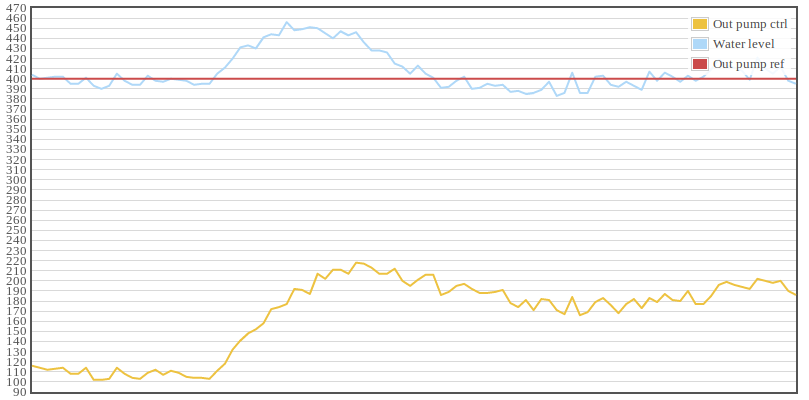
\includegraphics[width=1.0\textwidth]{plot1.png}
\caption{A PID client regulating the water level with the out pump with reference value 400.}
\label{fig:out pump}
\end{figure}

When running the server and a HTTP client (serving the plot system) on a
Raspberry Pi serving plots to two clients and having one manual control client
and one PID client the system use was about 3 \% CPU usage by the server and 
about 30 \% CPU usage by the HTTP server.


\subsection{Delay Measurements of the System}
Doing ten thousand get and set request via the driver to find the delay; a ping test was also done: 
\begin{itemize}
\item{Set: 0.133 ms}
\item{Get: 0.390 ms}
\item{Ping: 0.4 ms} 
\end{itemize}

Note that there was only a switch to travel through for the ping request.


\section{Conclusion}
% A conclusion section.\ref{kokare.c}. 
The CPU usage shown in section \ref{results} indicates that there is no need of having
the system spread out over multiple devices even if the system is designed to be spread out over
multiple devices.

The delay of the system is too small to create a problem. Even with greater distances between the client and the server, the delay would not pose a problem since the batch tank process is too slow.

The derivative part of the controller could not be used because it only
amplifies the high frequency noise observed.

\newpage

\begin{thebibliography}{9}
\bibitem{repo}
Project source code
\url{https://github.com/Fulkerson/FRTN01}
\bibitem{clientserver}
Kusarige, V. (2006), \emph{Client/server technology}, Southern Connecticut State University.
\bibitem{json}
JSON\\
\url{http://www.json.org}
\bibitem{python}
Python\\
\url{http://python.org}
\bibitem{project12}
Real-Time Systems: Project Descriptions 2012\\
\url{http://www.control.lth.se/media/Education/EngineeringProgram/FRTN01/2012/projects12.pdf}
\bibitem{kokare.c}
\url{cook/kokare.c}
\bibitem{protobuf}
Protocol Buffers\\
\url{http://code.google.com/p/protobuf}
\bibitem{rtcs}
Årzén, KE. (2012) \emph{Real-Time Control Systems}, Department of
Automatic Control, Lund University.
\bibitem{boost::asio}
boost::asio\\
\url{http://www.boost.org/doc/libs/1_52_0/doc/html/boost_asio.html}
\bibitem{boost::thread}
boost::thread\\
\url{http://www.boost.org/doc/libs/1_52_0/doc/html/thread.html}
\end{thebibliography}

\end{document}
